% !TeX root = ../main.tex

\chapter{问题分析}

假设 $a>0$,求解如下问题 (\ref{problem}) 的最优解:
\begin{equation}
  \min_{x\in\mathbb{R}}\frac{a}{2}x^2+dx+\sum^{m}_{i=1}\max(0,b_ix+c_i)\label{problem}
\end{equation}

要求解问题 (\ref{problem}),即求解如下问题 (\ref{fx}) 的最优解 \cite{10.1016/j.patcog.2017.02.006},其中 $I(b_ix+c_i)=\{b_ix+c_i\ge0\}$:
\begin{align}
  f(x)
   & =\frac{a}{2}x^2+dx+\sum^{m}_{i=1}\max(0,b_ix+c_i)\nonumber           \\
   & =\frac{a}{2}x^2+dx+\sum_{i\in I(b_ix+c_i)}\max(0,b_ix+c_i)\label{fx}
\end{align}

要求解问题 (\ref{fx}),我们可以对问题 (\ref{fx}) 求次梯度函数:
\begin{align}
  g(x)
   & =\partial f(x)\nonumber                    \\
   & =ax+d+\sum_{i\in I(b_ix+c_i)}b_i\label{gx}
\end{align}

根据图 (\ref{SubGradient}) 不难看出,$g(x)$ 是由如下断点集合分割的一个分段函数:
\begin{equation}
  x=\{x_i|x_i=-\frac{c_i}{b_i},i=1\dots m\}\nonumber
\end{equation}

次梯度函数 $g(x)$ 图像如图所示:
\begin{figure}[htb]
  \centering
  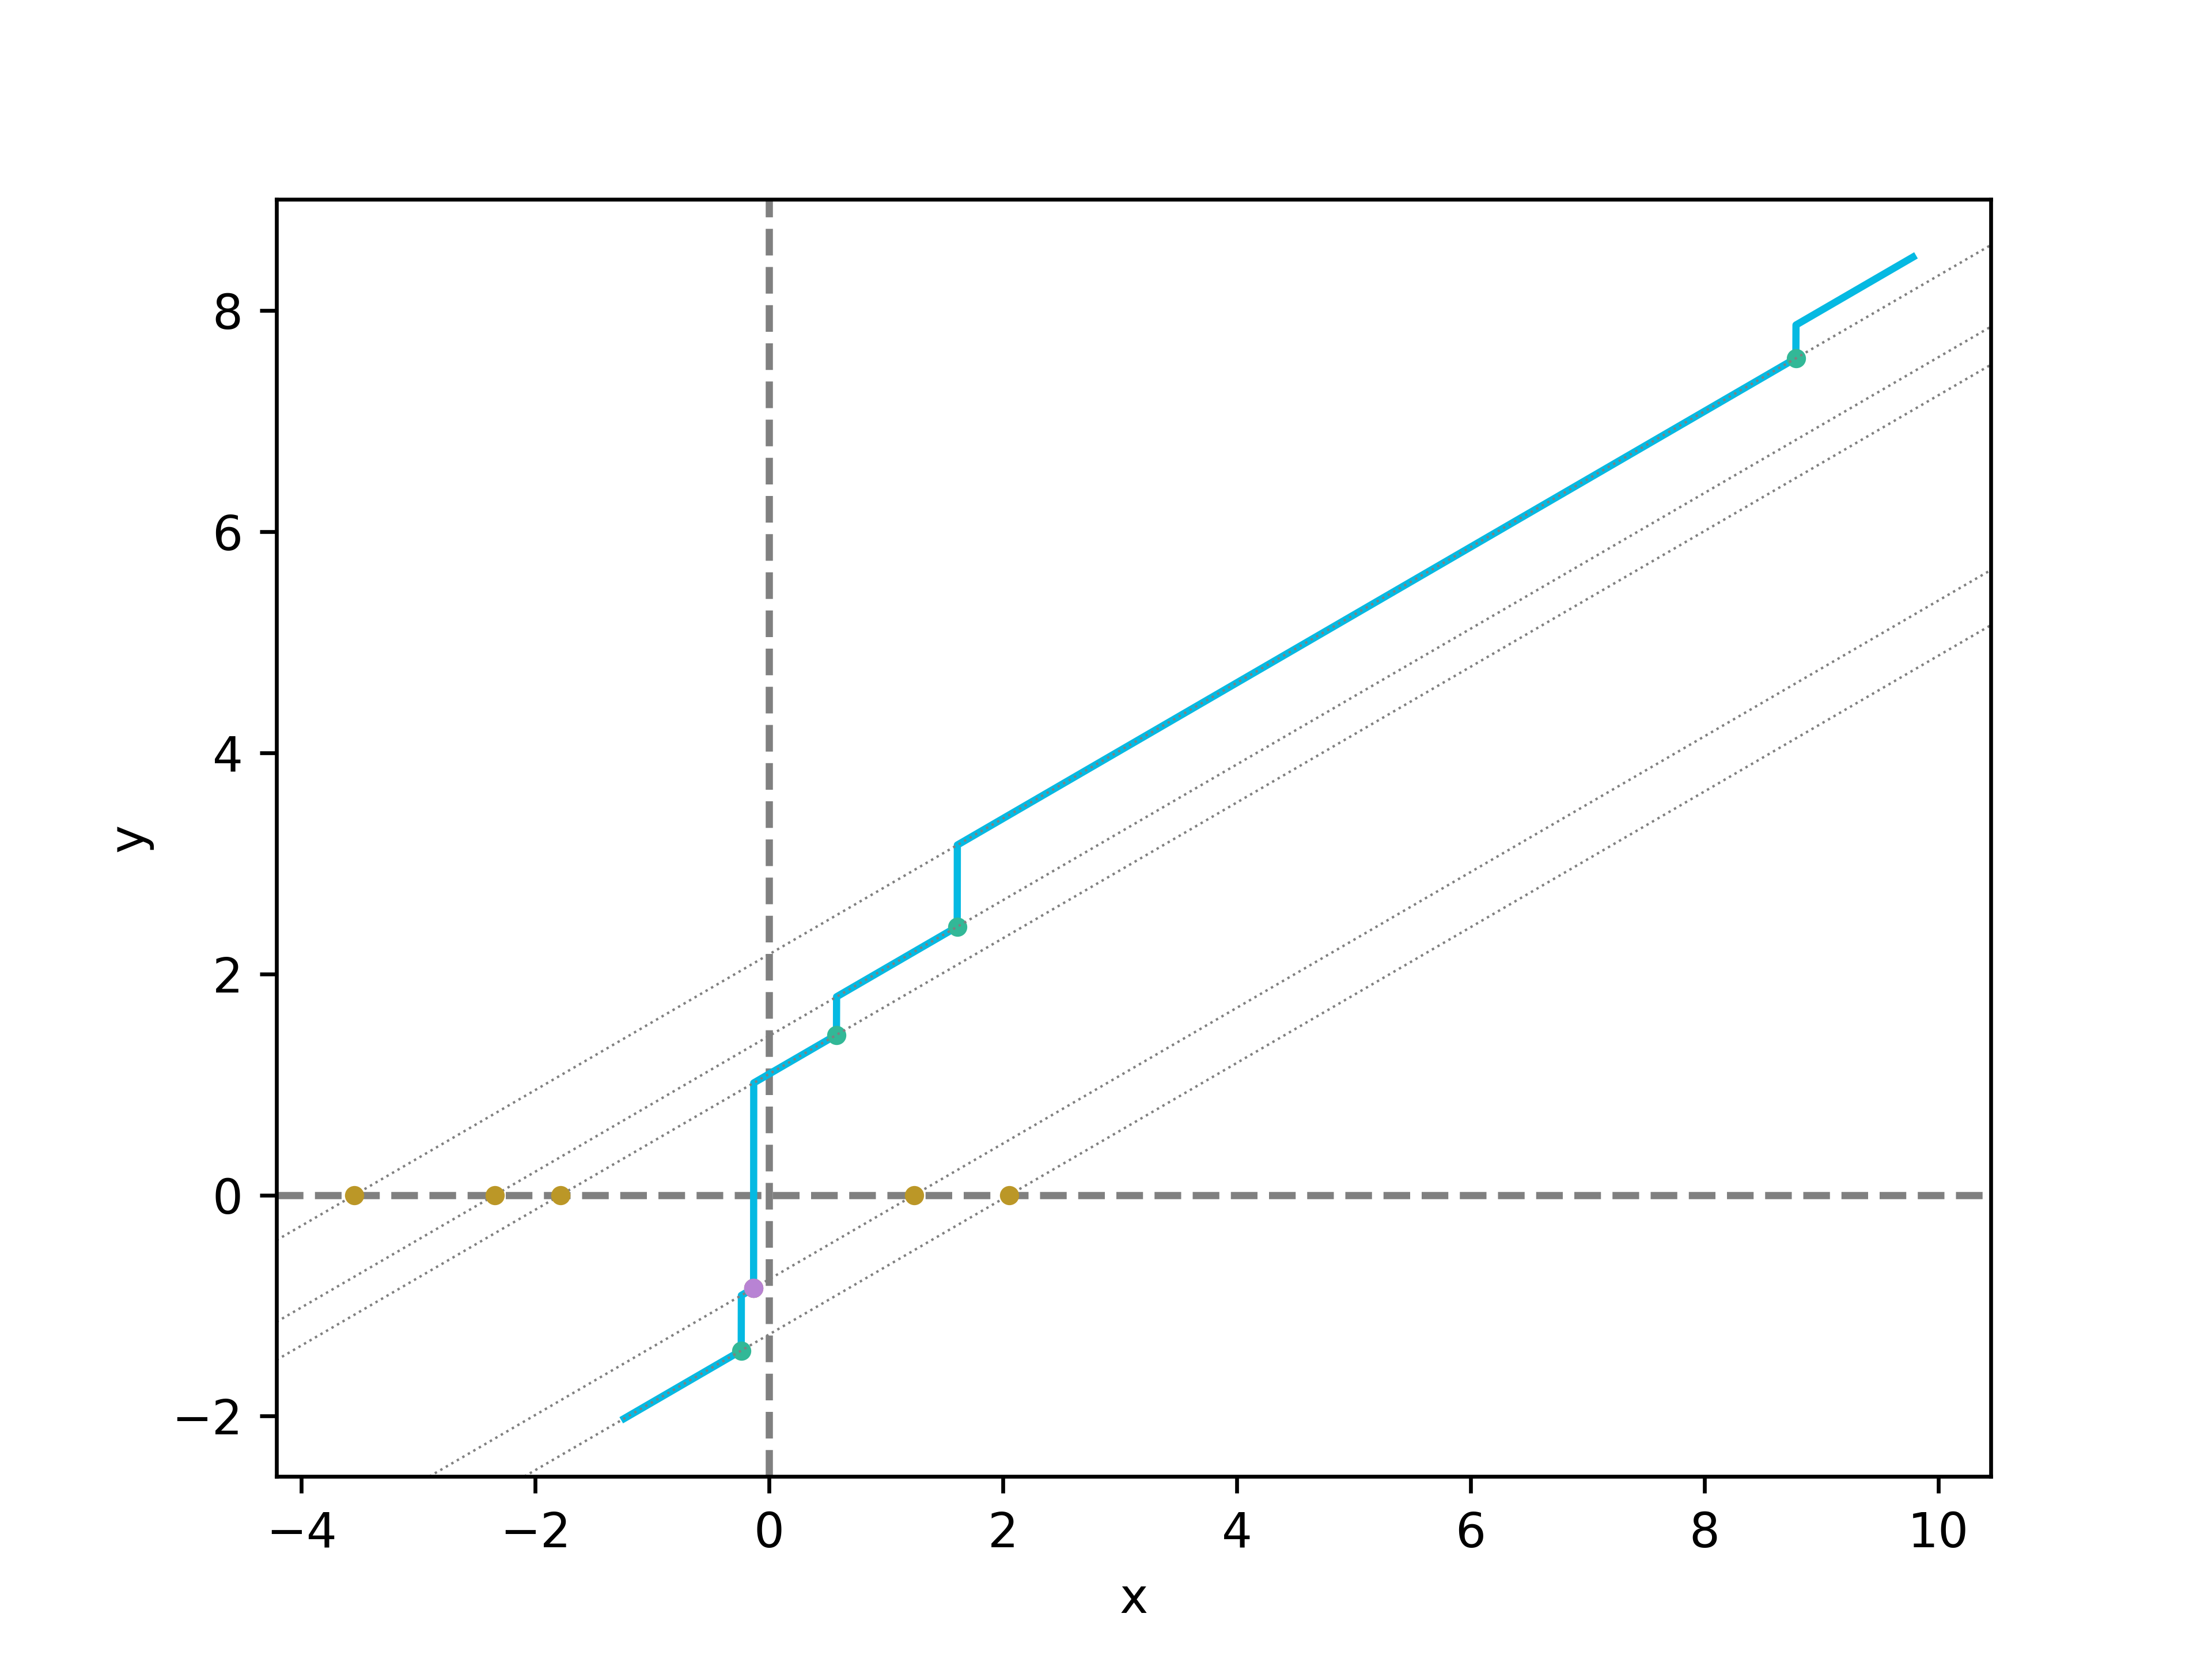
\includegraphics[width=0.5\textwidth]{figures/SubGradient.png}
  \caption{次梯度函数图像}
  \label{SubGradient}
\end{figure}

此时我们所要求的问题 (\ref{problem}) 转换为了求解一 $x^*$ 使得 $x^*\in\mathbb{R}$ 且 $0\in g(x^*)$。